\chapter{Machine Learning Approach}
\section{Background}
A random forest is a type of supervised classification or regression model, it is comprised of multiple decision trees 
that are combined to produce a single result, in this project we use it to classify sample points of an ECG 
Signal as either an QRS complex or not \cite{Kavlakoglu2021}. Decision trees can be thought of as a tree like flowchart, 
where you evaluate yes or no conditions at each node, where a yes or no correspond to a seperate branch leading to 
a new condition to evaluate, or a final result. The idea of decision trees is to seek the best split of the data, against
there trained classification data \cite{Kavlakoglu2021}. A random forest, trains each of these trees utilising a 
bootstrap aggregation method, where multiple training subsets a created with replacement, and each decision tree is 
trained independently on these subsets and with feature randomness, that is on a random subset of features, to ensure low correlation of the trees (i.e each tree 
isn't doing the same thing) \cite{Kavlakoglu2021}. The final result of the Random forest is chosen as the majority 
value (i.e yes or no). 

\section{QRS Identification}
We train the model on the first 15 mins of data associated with the datasets: a01, a12, a13, x04, a03, b01, b02. 
The reasoning for choosing these sets is in section 2 we saw they capture the varying morphology of ECG signals. 
The data features inputed into the models are the ECG data, derivative, derivative squared, second derivative, 
Processed Signal (from section 4), and Frequency filtered (5 - 35Hz) data. The motivation behind choosing 
these features is that they should change for QRS peaks, which can be thought of as large gradient changes, 
whilst the Process and Filtered Signal help ensure the model is robust against the presense of noise. The training 
labels for these sets are created from the annotation files, where each data sample recieves as 0 value, unless 
it is located at the annotation value or 2 samples either side, to provide the model with some cushioning to capture 
the changing behaviour associated with a peak. The model is built using Scipys RandomForestClassifer, 
chosen with the following hyperparameters, 100 estimators (i.e decision tress), max tree depth of 30
and with balanced class weight. \\

To evaluate the performance of the model we test it against ECG data from the 60-65th minute of the same dataset. 
We first test its performance against the labelled data associated with annotation files using the Precision, Recall and F1 metrics,
which are defined as follows. Let $TP$ denote true positives i.e how many predicted (1s) are actually (1s), 
let $FP$ denote false positives i.e how many predicts (1s) aren't acutally (1s) and let $FN$ denote 
the number of 1s that weren't detected. \\ 
Precision is the porportion of predicted 1s that are acutally 1s, i.e how many samples that are predicted
as part of a QRS complex, actually are part of a QRS compelex. 
\[
\text{Precision} = \frac{TP}{TP + FP}.
\]
Recall is the proportion of 1s that are detected, i.e the proportion of samples that are part of the QRS complexes, 
that have been detected. 
\[
\text{Recall} = \frac{TP}{TP + FN}.
\]
The F1 score is a balanced metric to capture both Precision and Recall, its specifically the harmonic mean of each.
\[
\text{F1} = 2 \times \frac{\text{Precision} \times \text{Recall}}{\text{Precision} + \text{Recall}}.
\]

\begin{table}[H]
    \centering
    \caption{Precision, Recall and F1 metric values for each dataset from 60-65min.}
    \label{tab:model_metrics}

    \csvautobooktabular{results_model_metrics.csv}
\end{table}
In Table~\ref{tab:model_metrics} we can see that the model has strong Precision scores from 0.92 - 1.0, 
however the Recall scores aren't great, with some as little as 0.25, suggesting the model is precise, 
that is when it recognises a sample as part of a QRS complex it often is, but isn't as strong at locating 
all samples that are apart of a QRS complex. \\

The performance above is tested against recognising samples that are apart of QRS complexes, for this project we are more 
focused on identifying the occurence of a complex. We convert the predicted samples to identify
occurence of complexes, by recognising clusters of 1s including patterns such as 1101 as a peak and choosing 
the middle value as the location.  In Table~\ref{tab:model_ann_scores}, we calculate the proportion of matching 
peaks, along with number of hallucinated and missed peaks for this approach. The results show strong performance, 
with very few hallucinated or missed peaks, and a large proportion of peaks matched across all datasets.  
\begin{table}[H]
    \centering
    \caption{Proportion of peaks found, peaks hallucinated and peaks 
    missed by model for each dataset from 60-65min.}
    \label{tab:model_ann_scores}
    \csvautobooktabular{results_model_annscores.csv}

\end{table}

\section{Respiratory Estimation}

In Section 5.2 we saw very promising signs for the performance of the Random Forest model, so we decide to explore 
its ability to detect trends when using RSA with FFT implementation, as we saw that was the most effective approach. 
In Figure ~\ref{fig:RSA_files_fft_model}, we can see that the model is able to predict distinct trends in 
the expected Respiratory Rate range in x04, b01 and a13 along with less distinct pattern in a01. This shows 
promising signs for the viability of a RSA based Respiratory Rate estimation method, implementing machine learning to 
detect peaks. 
\begin{figure}[H]
    \centering
    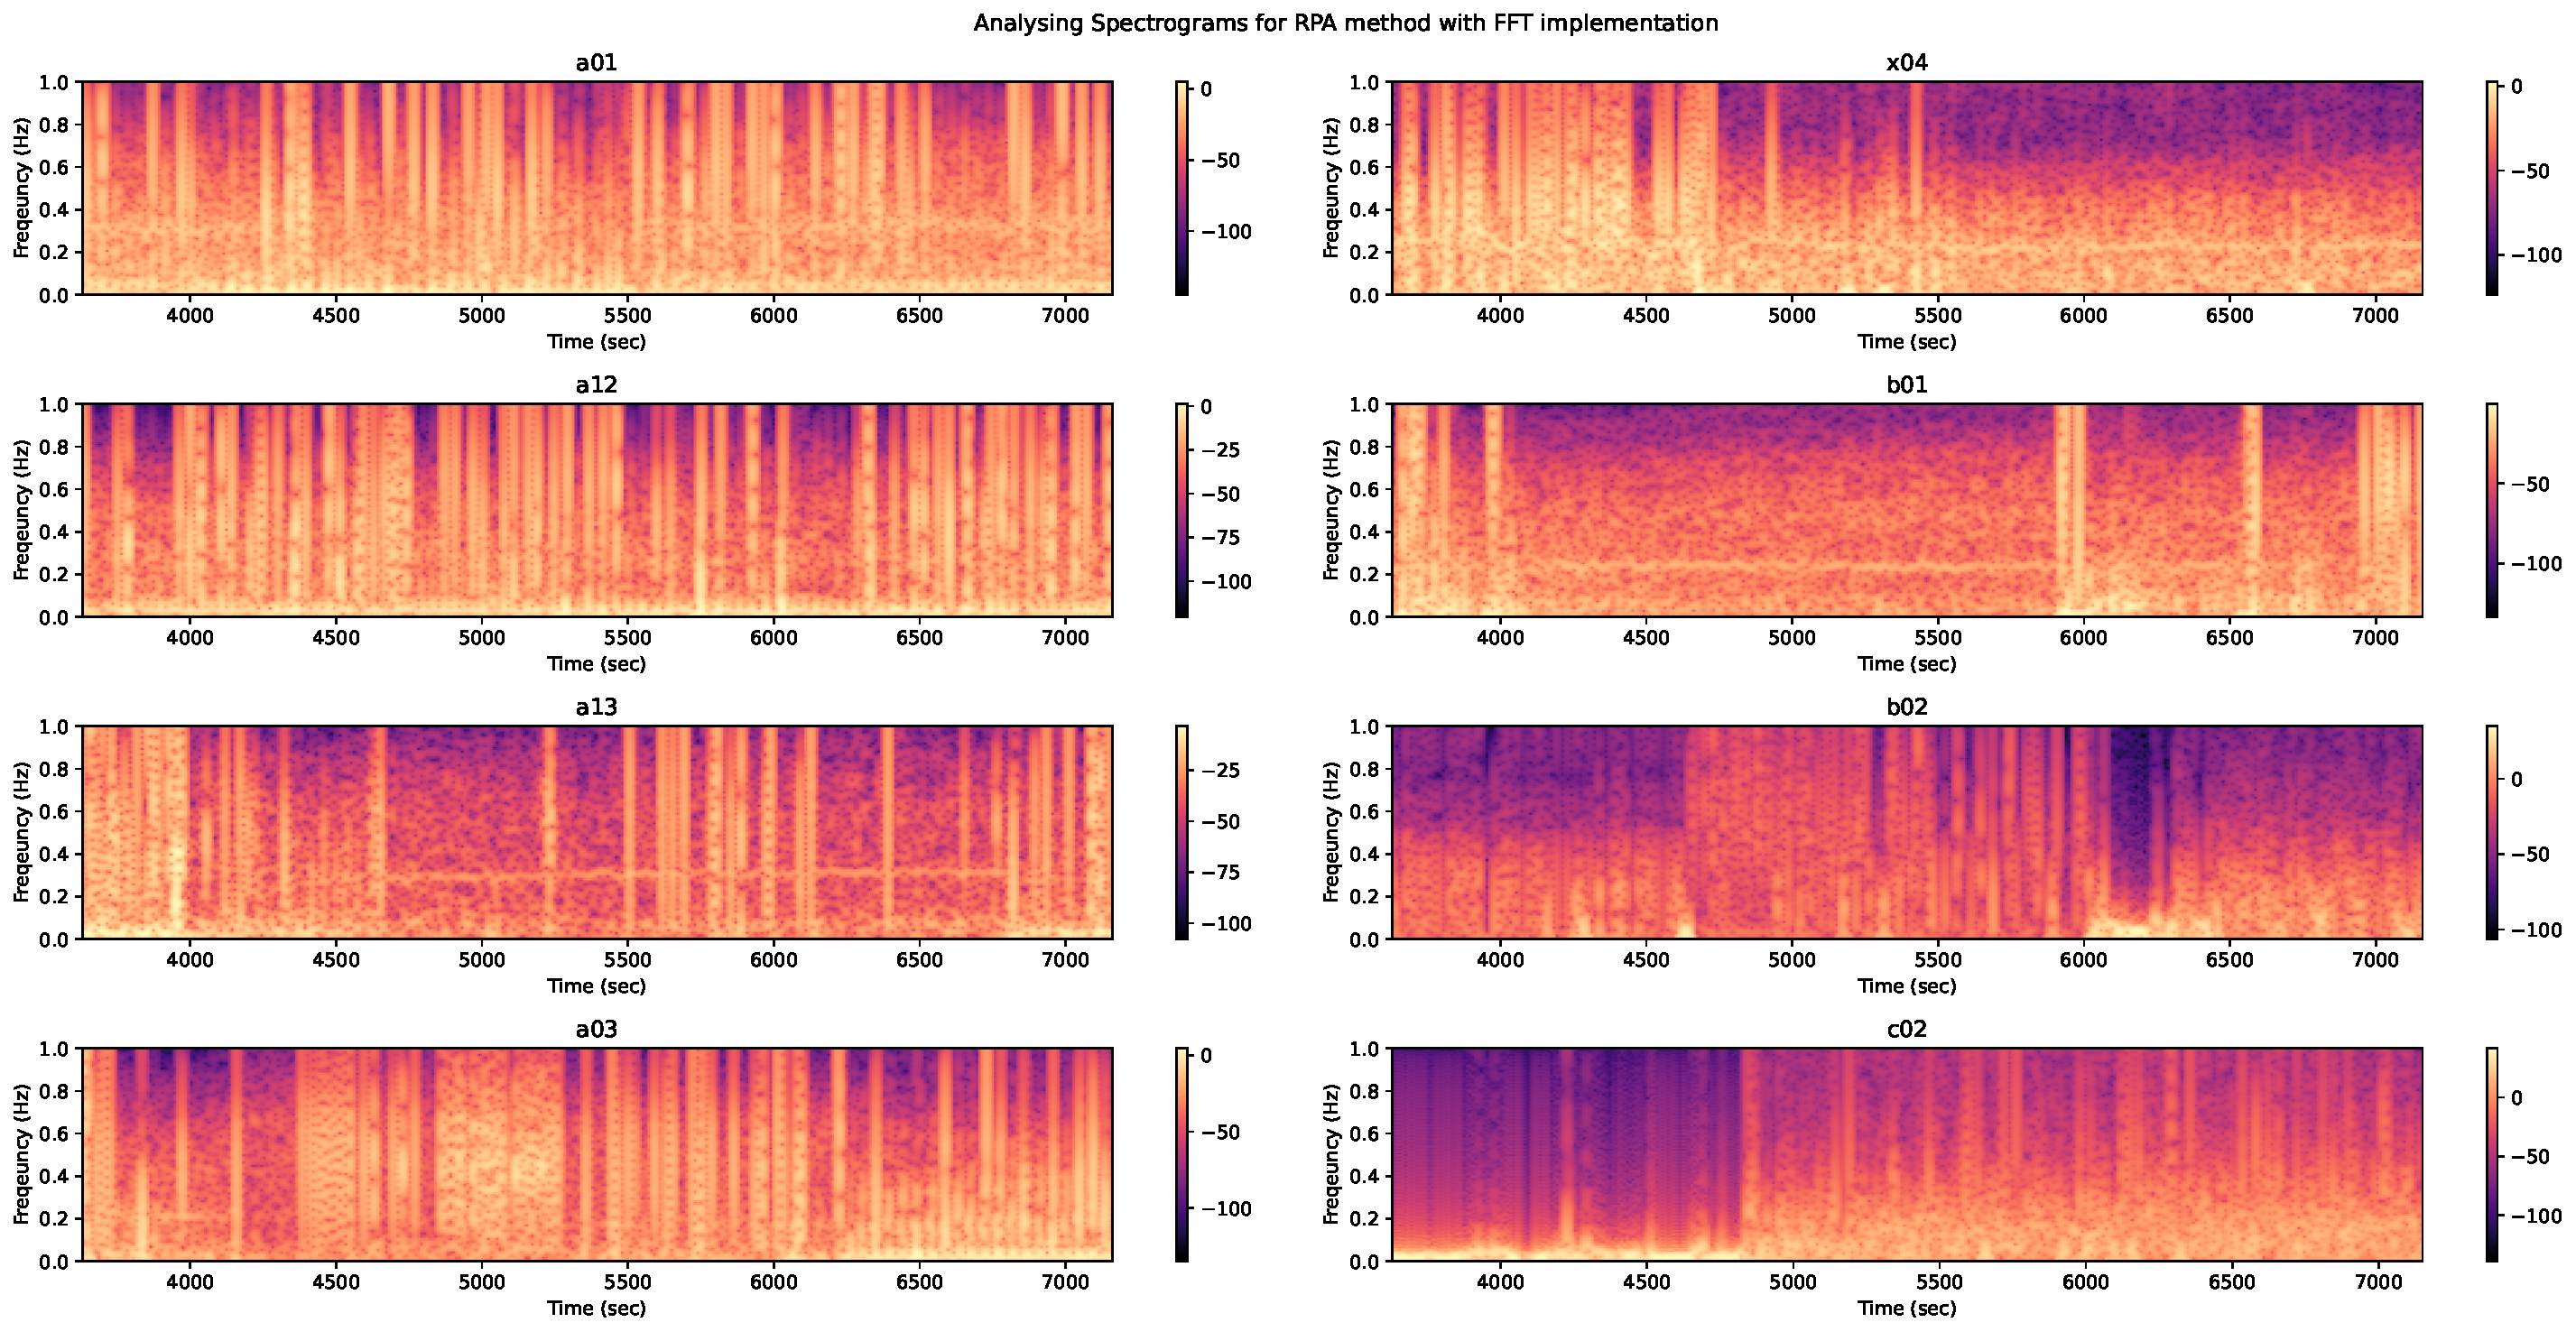
\includegraphics[width=\textwidth]{figures/RPA_spectrogram_files_FFT_mlmodel.pdf}
    \caption{Spectrogram comparison across datasets for RSA method with FFT implementation 
    with peaks identified with the Model.}
    \label{fig:RSA_files_fft_model}
\end{figure}

In order to ensure that the trends above weren't artifacts of the Machine Learning Model, we plot 
the RSA waveforms with peak data from the Jump Algorithm, Annotation Algorithm and Machine Learning Model, 
as shown in Figure~\ref{fig:RSA_methods}. 
\begin{figure}[H]
    \centering
    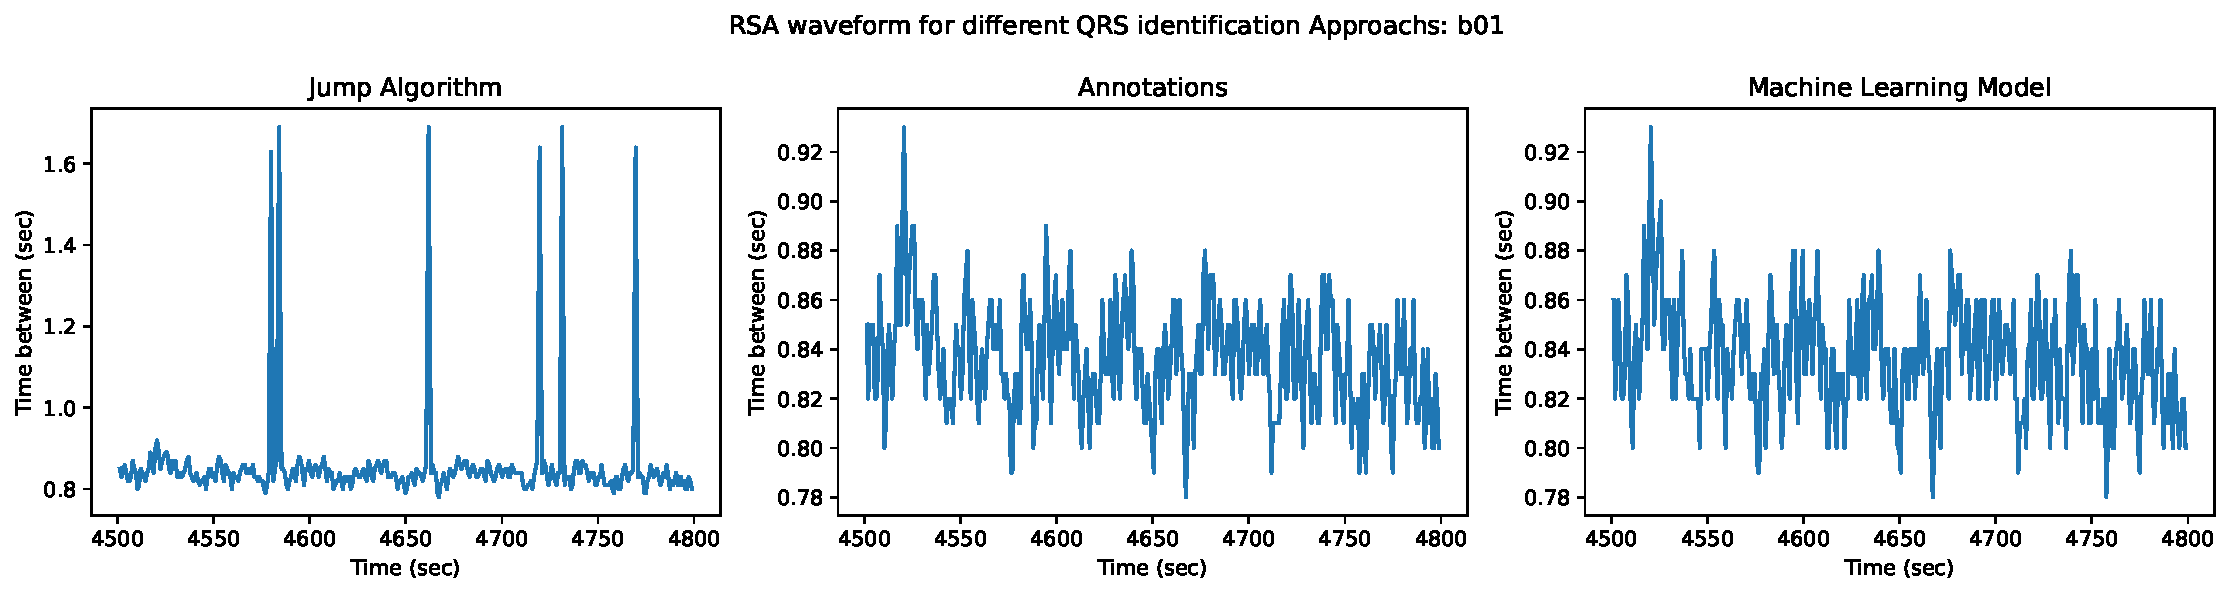
\includegraphics[width=\textwidth]{figures/RSA_data_peak_method_comp.pdf}
    \caption{Plot comparing RSA waveform utilising different peak identifcation methods.}
    \label{fig:RSA_methods}
\end{figure}

In Figure~\ref{fig:RSA_methods} we can see the clear wave like behaviour of the RSA data for all three methods, 
validating our spectrum approach, we can see a few artificats in the jump waves, however all three 
have similiar form. This is a strong indication that the trends in  Figure~\ref{fig:RSA_files_fft_model} aren't 
an artificat as the plot illustrates the wave in a range where a strong trend is identified, and matches 
closely to that of the annotations, however this trend isn't seen in the annotations illustrating the ability of the
model to highlight trends. 